
\documentclass[journal]{IEEEtran}
\usepackage[section]{placeins}
\usepackage{blindtext}
\usepackage{graphicx}
\usepackage{caption}
\usepackage{amsmath}
\usepackage{hyperref}
\usepackage{mwe}
\usepackage[options]{algorithm2e}


\ifCLASSINFOpdf
\else
\fi
\hyphenation{Gender Identification}


\begin{document}
	%
	% paper title
	\title{Dictionary Based Filtering}
	
	\author{\thanks{Dr. Mehul Raval}\thanks{Mr. Vibhav Joshi} Charvik Patel,~\IEEEmembership{1401079},
		Himanshu Budhia,~\IEEEmembership{1401039},
		Neel Puniwala,~\IEEEmembership{1401024}, 
		Maharsh Patel,~\IEEEmembership{1401109}}
	
	
	
	
	% make the title area
	\maketitle
	
	
	\begin{abstract}
		%\boldmath
		Digital image processing refers to the process of digital
		images by means of digital computer. The main application
		area in digital image processing is to enhance the pictorial
		data for human interpretation. In image some of
		the unwanted information is present that will be removed by
		several preprocessing techniques. Filtering helps to enhance
		the image by removing noise.Initially By creating Dictionary we will store two form of matrix.now when We add new image in dictionary we don't need to pass image from filter instead we will just Dictionary Learn form the Previous Dictionary and just map into.
		
	\end{abstract}
	\begin{IEEEkeywords}
		Dictionary Learning,Low-pass filter,Salt-Pepper Noise,Median filter
	\end{IEEEkeywords}
	
	
	\IEEEpeerreviewmaketitle
	
	
	
	\section{\textbf{Introduction}}
	Basically the idea of Dictionary based filtering is instead of doing classical convolution every time,we directly take de\textendash noise image from the dictionary using searching algorithm and time after time Learning of dictionary is also done by the same algorithm. We are planning to do low pass or high pass filtering to de\textendash noise the noisy image. Low pass filter is used to remove salt and paper noise while high pass filter is used to separate of edges.We use OpenCV libraries and Python libraries to implement the low pass filter and to create blocks of image.
	
	Initially we take some training and filter them by using classical convolution.Both filtered and non-filtered images are divided into blocks which are stored in a dictionary.In the dictionary the key is noisy part of the image and the value is filtered part of the image.
	
	\section{\textbf{Methodology}}
	\begin{minipage}{\linewidth}
		\centering
		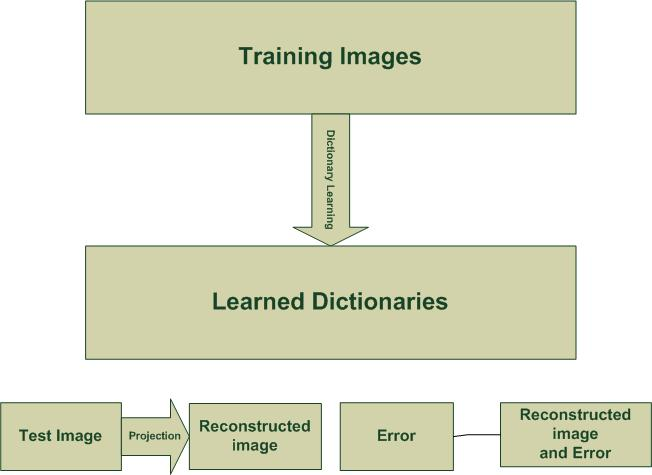
\includegraphics[width = 80mm]{2.jpg}
		\captionof{figure}{Methodology[3] \label{overflow}}
	\end{minipage} 
	\section{\textbf{Literature review}}
	\subsection{\textbf{Salt and Pepper Filtering}}
	Salt-and-pepper noise is a form of noise sometimes seen on images. It presents itself as sparsely occurring white and black pixels. An effective noise reduction method for this type of noise is a median filter.[2]\\
	  In Median Filter,
	 The original pixel values and the values replaced by their median are shown side by side below\\
	\begin{minipage}{\linewidth}
		\centering
		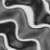
\includegraphics[width = 80mm]{1.jpg}
		\captionof{figure}{Median Filter Conversion[1] \label{overflow}}
	\end{minipage} 
		
	From the above illustration it is clear that the pixal value '128' is replaced by the median value 24 and the pixel value '172' is replaced by the median value 31. here the values 128 and 172 are entirely different from their neighboring pixels. when we take the median value,the pixel values which are totally different from their neighboring pixels are replaced by a value equal to the neighboring pixel value. hence Median Filter will reduce salt-pepper noise of image. 
	\subsection{\textbf{Sparse Dictionary Learning}}[5]
	Sparse dictionary learning is a representation learning method which aims at finding a sparse representation of the input data (also known as sparse coding) in the form of a linear combination of basic elements as well as those basic elements themselves. These elements are called atoms and they compose a dictionary. Atoms in the dictionary are not required to be orthogonal, and they may be an over-complete spanning set. This problem setup also allows the dimensionality of the signals being represented to be higher than the one of the signals being observed.
	
	One of the key principles of dictionary learning is that the dictionary has to be inferred from the input data. The emergence of sparse dictionary learning methods was stimulated by the fact that in signal processing one typically wants to represent the input data using as few components as possible.
	
	Different Algorithm for Sparse Dictionary Learning are as follow.
	\begin{enumerate}
		\item Method of optimal directions (MOD)
		\item K-SVD[4]
		\begin{enumerate}
			\item K-SVD method learns an over-complete
			dictionary from an input image via solving the following minimization model
			\item \textbf{Limitation:}Choosing an appropriate "dictionary" for a dataset is a non-convex problem, and K-SVD operates by an iterative update which does not guarantee to find the global optimum.
			
		\end{enumerate}
		\item Stochastic gradient descent
		\item Parametric training methods
		\item Online dictionary learning
	\end{enumerate}
	\subsection{\textbf{Flow of Implementation}}
	
	
	\begin{algorithm}
	First of all we have to take n x n training
	image.\\
		Create m x m blocks.\\
		Create dictionary using blocks.\\
		Dictionary:\\
		\hspace{1cm}	 \textbf{Key} - Noisy image\\
		\hspace{1cm}	 \textbf{value} - filtered image\\
		Search algorithm\\
			\eIf{Nearest Possible Match}{
				Noisy Patch Replaced with this Image
     		}{
			Add to Dictionary
		}
	return \textbf{Final Filtered Image}
	
\end{algorithm}

	


	
	\ifCLASSOPTIONcaptionsoff
	\newpage
	\fi
	
	\section{\textbf{Output}}
	    \begin{minipage}{\linewidth}
	    	\centering
	    	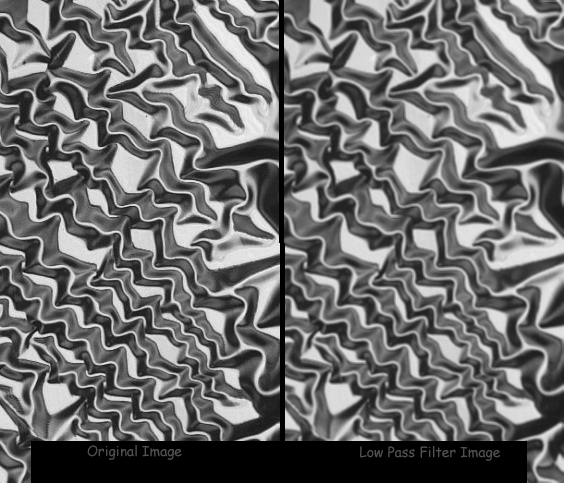
\includegraphics[width=80mm]{3.jpg}
	    	\captionof{figure}{Output \label{overflow}}
	    \end{minipage} 
	\section{\textbf{Conclusion}}
	We are successfully able to create m x m blocks from n x k dimension image where m $\ll$ n. We also have implemented low pass filtering. We take m = 3, 5, 7, 10, 50 and observe that, when m is very small we get more accurate result. Size of dictionary is inversely proportional to m. Therefore, there is always trade-off between accuracy of result and size of dictionary.   
	
	
    \section{\textbf{Future Work}}
    We are planning to implement efficient searching algorithm to search image from the dictionary and trying to compare running time of our algorithm (dictionary based approach) with running time of classical convolution approach.
	
	
	\begin{thebibliography}{8}
	\bibitem{IEEEhowto:kopka}
	“Digital Image Processing”, JAYARAMAN
	\bibitem{IEEEhowto:kopka}
	"Median filter", En.wikipedia.org, 2017. [Online]. Available: \url{https://en.wikipedia.org/wiki/Median_filter}. [Accessed: 03- Mar- 2017].
	\bibitem{IEEEhowto:kopka}
	"Dictionary-Based Face Recognition Under Variable
	Lighting and Pose",Vishal M. Patel,TaoWu,SomaBiswas,P. Jonathon Phillips,Rama Chellappa.[Accessed: 25- Feb- 2017].
	\bibitem{IEEEhowto:kopka}
   "K-SVD", En.wikipedia.org, 2017. [Online]. Available: \url{https://en.wikipedia.org/wiki/K-SVD}. [Accessed: 03- Mar- 2017].	\bibitem{IEEEhowto:kopka}
"Sparse dictionary learning", En.wikipedia.org, 2017. [Online]. Available:\url{https://en.wikipedia.org/wiki/Sparse_dictionary_learning}	[Accessed: 25- Feb- 2017].
\bibitem{IEEEhowto:kopka}
A.  Rosebrock, "Convolutions with OpenCV and Python - PyImageSearch", PyImageSearch, 2017. [Online]. Available:\url{ http://www.pyimagesearch.com/2016/07/25/convolutions-with-opencv-and-python/}. [Accessed: 01- Mar- 2017].

\bibitem{IEEEhowto:kopka}
"How to Split Image Into Multiple Pieces in Python", Stackoverflow.com, 2017. [Online]. Available: \url{http://stackoverflow.com/questions/5953373/how-to-split-image-into-multiple-pieces-in-python}. [Accessed: 01- Mar- 2017].

\bibitem{IEEEhowto:kopka}
[4]"Image denoising using dictionary learning — scikit-learn 0.18.1 documentation", Scikit-learn.org, 2017. [Online]. Available: \url{http://scikit-learn.org/stable/auto_examples/decomposition/plot_image_denoising.html}. [Accessed: 01- Mar- 2017].

	
	\end{thebibliography}
	
	
	
\end{document}


